\subsubsection{Eliminierung 3 bis 21 Harmonischer}
Dieses Pulsmuster basiert auf dem selben Prinzip wie jenes im Kapitel \ref{6_2_title}. Jedoch werden hier die [3, 5, 7, 9, 11, 13, 15, 17, 19, 21] Harmonische eliminiert. Um zehn Harmonische zu eliminieren, benötigt man zehn Freiheitsgrade [$\alpha_1, \alpha_2, \alpha_3, \alpha_4, \alpha_5, \alpha_6, \alpha_7, \alpha_8, \alpha_9, \alpha_{10}$].\\
\\

\begin{figure}[H]
  \begin{center}
  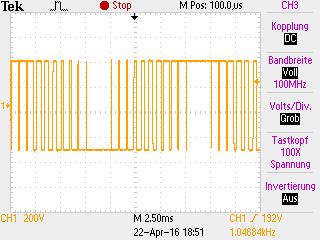
\includegraphics[width=0.48\textwidth]
  {pic/6_2_weitere_pulsmuster/6_2_1_stromform/eliminierung_3_bis_21/ALL0000/F0000TEK.png}
  \caption{$U_A (Orange)$}
  \label{fig:6_2_3_0}
  \end{center}
\end{figure}


\begin{figure}[H]
  \begin{center}
  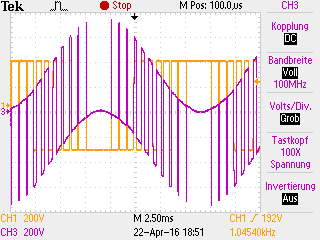
\includegraphics[width=0.48\textwidth]
  {pic/6_2_weitere_pulsmuster/6_2_1_stromform/eliminierung_3_bis_21/ALL0001/F0001TEK.png}
  \caption{$U_A (Orange), U_L (Violett)$}
  \label{fig:6_2_3_1}
  \end{center}
\end{figure}


\begin{figure}[H]
  \begin{center}
  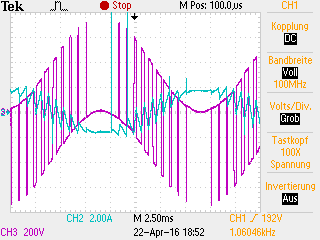
\includegraphics[width=0.48\textwidth]
  {pic/6_2_weitere_pulsmuster/6_2_1_stromform/eliminierung_3_bis_21/ALL0002/F0002TEK.png}
  \caption{$U_L (Violett), I_{L1} (Hellblau)$}
  \label{fig:6_2_3_2}
  \end{center}
\end{figure}
In dem Stromverlauf $I_{L1}$  ist nun eine klare Sinusform erkennbar.


\clearpage